\section{Introduction}
\section{Related Work}

\section{Concept}
\section{Implementation}
\section{Evaluation}
\section{Conclusion}




first level: section\\
second level: subsection\\
third level: subsubsection\\
fourth level: paragraph

\begin{table}[tbh!]
\caption{Table captions should be placed above the
tables.}\label{tab1}
\begin{tabular}{lll}
\hline
Heading level &  Example & Font size and style\\
\hline
Title (centered) &  {\Large\bfseries Lecture Notes} & 14 point, bold\\
1st-level heading &  {\large\bfseries 1 Introduction} & 12 point, bold\\
2nd-level heading & {\bfseries 2.1 Printing Area} & 10 point, bold\\
3rd-level heading & {\bfseries Run-in Heading in Bold.} Text follows & 10 point, bold\\
4th-level heading & {\itshape Lowest Level Heading.} Text follows & 10 point, italic\\
\hline
\end{tabular}
\end{table}
Displayed equations are centered and set on a separate line.
\begin{equation}
x + y = z
\end{equation}
Please try to avoid rasterized images for line-art diagrams and
schemas. Whenever possible, use vector graphics instead (see
Figure~\ref{fig1}).

\begin{figure}[tbh!]
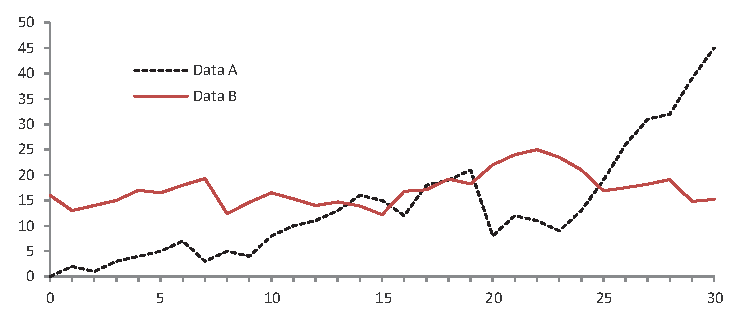
\includegraphics[width=\textwidth]{fig1.eps}
\caption{A figure caption is always placed below the illustration.
Please note that short captions are centered, while long ones are
justified by the macro package automatically.} \label{fig1}
\end{figure}
